%Notes: Add more description in demonstration section
%Pull more specifics from the powepoint, also more
%description on the proxy overhead paper
\chapter{An Inexpensive Testbed for Mobile Device Power Measurement} 
\label{ch:testbed}


\section*{Introduction}
%addcontentsline add section to table of contents
\addcontentsline{toc}{section}{Introduction}

Over the last few decades, there has been an enormous increase in the ubiquity of mobile devices. With this increase, has also come the increase in demand for data-driven services and this demand is predicted to continue \cite{VNI14}. The battery consumption of mobile devices represents a limiting bottleneck and thus  power optimizations suggestions have been suggested \cite{Qian:2012:PTM:2187836.2187844}. Software-based energy profilers do exist \cite{DAmato:2011:EAE:2419622.2419929}, however they are not always feasible for implementing in a straightforward manner or desirable due to rapid development cycles. To overcome these barriers, a real world test bed that can be implemented which to perform measurement of power consumptions on mobile devices.

\addcontentsline{toc}{section}{Hardware Configuration}
%Putting an asterisk after section leaves out the II. formatting
\section*{Hardware Configuration}

The main component in this testbed is the mobile device.
This can be realized by using a smartphone and replacing the
battery with connectors to the power supply; alternatively one
of the common development board packages, such as
Pandaboard (see www.pandaboard.org) or Wandboard (see
www.wandboard.org) packages. Development boards and smartphones were utilized together with the
Android operating system, which provides log output via USB
to the measurement control device, which can be a regular PC
or another development board with Android debugging
support. The mobile device is then networked with a wireless access point, which allows for wired and wireless evaluations.
The switchable power supply has an external serial or USB
port to communicate the current and power in small time
intervals to the control device. A BK Precision
1696 switchable power supply is utilized, as it offers fine granularity in power, current, and time intervals. While other equipment, such as Arduino with custom circuits, were used in other measurement approaches, these power supplies are common lab equipment and offer overall robust features.

\addcontentsline{toc}{section}{Software Configuration}
\section*{Software Configuration}
The software components are comprised of several Python scripts that execute the Android Debugging Bridge (ADB) and capture the output either to a local file or allow sending the output to a remote receiver, as illustrated in  Figure \ref{fig:testbed_setup}. The scripts allow for easy customization on the locally connected control device or at a remote location, e.g., filtering by specific events in the log. Similarly, a locally executing script captures the output from the power supply and is enabled to forward the data to a remote location as well.

\begin{figure}
\centering
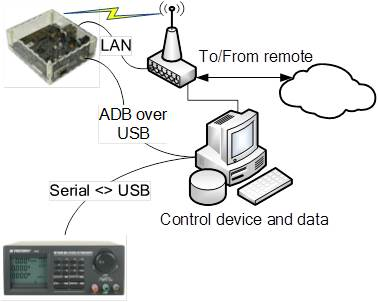
\includegraphics[scale=1,keepaspectratio]{testbed_setup}
\caption{Illustration of measurement testbed.}
\label{fig:testbed_setup}
\end{figure}

\addcontentsline{toc}{section}{Demonstration Description}
\section*{Demonstration Description}
To demonstrate the usefulness of the testbed, two different aspects of the measurement setup were utilized using an example Android application that performs web requests. This application makes requests to a local proxy server either serially or in parallel and the proxy server goes out and fetches what the phone requested.  The workflow for the application ca be seen in figure \ref{fig:testapp_workflow}. Both, wired and wireless access scenarios were exhibited for accessing a remote web service and retrieving results in order to demonstrate the functionality of the testbed. With these demonstrations, real time visualizations of the data about power consumption were created and stored on log files on a remote computer where they can be readily parsed for automatic evaluation  of application power consumption.

\begin{figure}
\centering
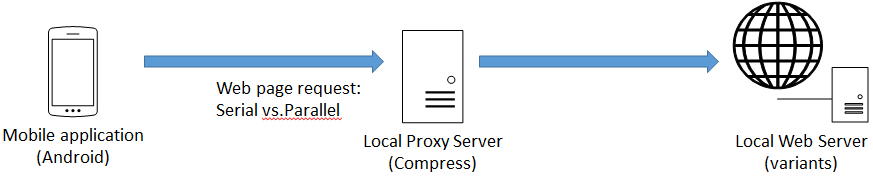
\includegraphics[scale=1,keepaspectratio,width=\textwidth]{testapp_workflow}
\caption{Workflow of mobile application tested on testbed.}
\label{fig:testapp_workflow}
\end{figure}
